%%%describing the basic usage

This chapter deals with the basic interface provided by the layer 1 types
implemented in \libpniio. All types concerning Nexus reside in one of the
namespaces embedded in \texttt{pni::io::nx}. The namespaces below this one 
indicate either a particular storage backend (currently only HDF5 is
implemented).

To use the Nexus part of the library just add 
\begin{cppcode}
#include <pni/io/nx/nx.hpp>
\end{cppcode}
to your source file. 

%%%===========================================================================
\section{Working with files}

\subsection{Creating single files}
The simplest approach towards handling \nexus-files is to create a single file 
to store data. This can be achieved with the \cpp{create\_file} static member 
function of \cpp{nxfile}.
\begin{cppcode}
#include <pni/io/nx/nx.hpp>

using namespace pni::io::nx;

int main(int argc,char **argv)
{
    h5::nxfile file = h5::nxfile::create_file("test.nxs");
    //... code omitted ...
    file.close();

    return 0;
}
\end{cppcode}
The code should be rather self explaining.  If the file already exists a
\cpp{object\_error} exception is thrown. 
In order to overwrite an existing file one can use
\begin{cppcode}
h5::nxfile file = h5::nxfile::create_file("test.nxs",true);
\end{cppcode}
where the second argument to \cpp{create\_file} enables overwriting an existing
file of same name. This option should be used with case as all data stored in 
the original file will be lost forever. 

\subsection{Create distributed files}
In cases where a single data file would grow rather large (more than $40$ GByte
for instance) creating a single large file is not a good solution. One problem
is the transfer of the file via the network. It would require a quite
sophisticated down- or upload software which must be able to recover a transfer
from a broken network connection, for instance. 
The other problem comes from archives. Data which should be archived goes
typically to a tape library. However, such libraries typically want to have
files in a particular size in order to operate with optimal performance. 

\libpniio\ allows the content of a single file to be distributed over several
files each having the same size. Such a set of files can be created using the 
\cpp{create\_files} static member function as shown below
\begin{cppcode}
h5::nxfile file = h5::nxfile::create_files("test.%04i.nxs",1024);
\end{cppcode}
Aside from its name the arguments of the \cpp{create\_files} function have 
a slightly different meaning. If a set of files should be produced the file name
is not a simple string but a \cpp{printf} like format string. This allows the
storage backend of \libpniio\ to number each new file as it is created.
The second argument to this function is the size in MByte an individual file can 
attain before a new one will be created. The above call to \cpp{create\_files}
would yield the following files
\begin{minted}{bash}
test.0001.nxs
test.0002.nxs
test.0003.nxs
...
\end{minted}
As for the simple \cpp{create\_file}, \cpp{create\_files} will throw an
\cpp{object\_error} exception if a file already exists. In order to overwrite an
existing file append \cpp{true} to the above call 
\begin{cppcode}
h5::nxfile file = h5::nxfile::create_files("test.%04i.nxs",1024,true);
\end{cppcode}
However, in this case already existing members of the family will not be removed
but just truncated (their size becomes $0$). So do not wonder that you still
find all the member files of a set even after overwriting it. Their size will be
set to zero.

%%%===========================================================================
\subsection{Opening and closing files}

If a file already exist the {\tt open\_file} static member function of the
\nxfile\ should be used.  Its signature is rather simple 
\begin{cppcode}
open_file(const string &n,bool ro=true)
\end{cppcode}
where the first argument is the name of the file and the second determines
whether or not the file will be opened in read-only mode. By default files are
opened read-only in order to avoid accidental changes in the file. 

\texttt{open\_file} can be used with a single file as well as with a file
family. For a single file use 
\begin{cppcode}
h5::nxfile f = h5::nxfile::open_file("test.nxs");
\end{cppcode}
In order to open a file split into several parts only a different file name 
must be used
\begin{cppcode}
h5::nxfile f = h5::nxfile::open_file("test.%05i.nxs");
\end{cppcode}
Like for file creation, the printf-like format string has to be used for the 
filename. 

Like all objects in \libpniio\ a file object is destroyed automatically if it
looses scope.  However, in some cases one may wants to explicitly close the
file. This can be done with the \texttt{close} member function
\begin{cppcode}
h5::nxfile f = ...;
.... code omitted ...
f.close();
\end{cppcode}

%%%===========================================================================
\subsection{Other file related functions}

Like virtually all level $1$ objects in \libpniio\ \nxfile\ posses an
\cpp{is\_valid} inquiry method. It can be used to check whether or not an
objects is a valid instance or not. This is necessary as a default constructed
file is not a valid instance. 
\begin{cppcode}
h5::nxfile f = ...;
...code omitted ...
if(!f.is_valid())
    std::cerr<<"Something went wrong!"<<std::endl;
\end{cppcode}
You can also check whether a file is read-only or not by means of the 
\cpp{is\_readonly} member function 
\begin{cppcode}
h5::nxfile f = ...;
...code omitted ...
if(f.is_readonly())
    std::cerr<<"File is in read-only mode!"<<std::endl;
\end{cppcode}
As one can see from the API documentation, the interface of \nxfile\ is rather
simple. In order to do anything useful (like creating groups and fields) one 
has to obtain the root group of the file. This can be done with the 
\cpp{root} member function
\begin{cppcode}
h5::nxfile f = ...;
h5::nxgroup root = f.root();
\end{cppcode}
Finally there is an important member function named \cpp{flush}. Whenever
possible use this function to explicitly hand over data from the underlying
storage library to the operating system for writing.
\begin{cppcode}
h5::nxfile f =....;

while(measurement_running())
{
    //record data

    //flush the file
    f.flush();
}
\end{cppcode}




%%%===========================================================================
\section{Working with groups}

\nexus\ groups are instances of the \nxgroup\ template. They can be considered
as containers for fields and other groups and expose an STL compliant interface. 
To start working with groups in a file one hast to first obtain the root group 
with 
\begin{cppcode}
h5::nxfile file = h5::nxfile::open_file("test.nxs");
h5::nxgroup root = file.root();
\end{cppcode}

\subsection{Creating groups}

New groups are created by means of the \cpp{create\_group} member function of
\nxgroup
\begin{cppcode}
h5::nxgroup entry = root.create_group("scan_1","NXentry");
\end{cppcode}
This method takes two arguments where the first one is mandatory and denotes the
name of the group while the second one is optional and determines the
\nexus-class of the group. If the last argument is omitted a simple HDF5 group
is created (without an \cpp{NX\_class}  attribute).

Like files, groups are automatically destroyed when an instance looses scope,
but they can also be deliberately closed using their \cpp{close()} method.

%%%===========================================================================
\subsection{Accessing children}

Access to the direct children of a group instance is given via the 
\cpp{at()} method or the \cpp{[]} operator. Both accept either a numeric index 
of a child or its name as an argument. To loop over all children of the 
root group the following code could be used
\begin{cppcode}
h5::nxfile f = ....;
h5::nxgroup root = f.root();

for(size_t i=0;i<root.size();++i) std::cout<<root[i].name()<<std::endl;
\end{cppcode}
As for STL containers, the \cpp{size()} method returns the number of children 
of a group. To access a particular group via its name one can use
\begin{cppcode}
h5::nxfile f = ....;
h5::nxgroup root = f.root();

h5::nxgroup entry = root["entry"]; //alternatively root.at("entry");
\end{cppcode}
Unlike for STL containers both access variants (\cpp{at()} or \cpp{[]}) will 
throw an exception if a particular child could not be found or the index passed
exceeds the total number of children of the group. In addition to this simple 
access interface \nxgroup\ also exposes a fully STL compliant iterator 
interface. However, in order to use it some more deeper knowledge about 
\libpniio\ is required and thus this topic will be dealt with in
Section~\ref{section:group_iteration}.

%%%===========================================================================
\subsection{Other group related member functions}

Like files, groups posses an \cpp{is\_valid()} method which allows checking the 
state of a group. Similar to files, default constructed instances of \nxgroup\
are not valid. 
\begin{cppcode}
h5::nxgroup entry; 

if(!entry.is_valid()) std::cerr<<"The entry group is not valid!"<<std::endl;
\end{cppcode}
The getter methods \cpp{name()} and \cpp{filename()} return the name of the
group and the name of the file the group is stored in respectively.
Finally the \cpp{parent()} function returns the parent group of the a group.
In order to use the \cpp{parent()} member function a bit more extra care is 
used. When using the method in a simple way like 
\begin{cppcode}
h5::nxgroup p = other_group.parent();
\end{cppcode}
everything will be fine. However, when we want to use the return value of 
\cpp{parent()} as a temporary we have to do an explicit conversion to 
\cpp{nxgroup} like this
\begin{cppcode}
std::cout<<h5::nxgroup(entry_group.parent())<<std::endl;
\end{cppcode}
The reason for this is that \cpp{parent()} does not really return an 
instance of \cpp{nxgroup} but rather of \cpp{nxobject}. 
But \nxobject\ can be converted to \nxgroup\ safely. The reason 
for this behavior will be explained in detail in Section~\ref{section:nxobject}.




%%%===========================================================================
\section{Working with fields}

Fields are the basic data holding facilities in \libpniio\ and are represented
by instances of \nxfield. One can imagine a field as a multidimensional array 
stored on disk. Thus, it has quite similar properties than instances of 
\cpp{mdarray} in \libpnicore.  It is impossible to create a purely 
scalar field with \libpniio\ as every field should be extensible if required. 

%%%===========================================================================
\subsection{Creating fields}

Fields are created as children of a particular group instance. Creating fields
is a rather complex task as there are many options available so lets start with 
the simplest possible example
\begin{cppcode}
h5::nxgroup entry = root["entry"];
h5::nxfield field = entry.create_field<float32>("temperature");
\end{cppcode}
This creates a 1D field with a single element. This is as closest one can get 
to store a scalar value. The template parameter of the \cpp{create\_field}
method can be any type supported by \libpnicore.  For multidimensional fields
use 
\begin{cppcode}
h5::nxgroup entry = root["entry"];
h5::nxfield field = entry.create_field<float32>("temperature",shape_t{3,4});
\end{cppcode}
which will create a $2$-dimensional field with a shape of $(3,4)$ and a total
size of $12$ elements.
When using HDF5 as a storage format a compression algorithm can be associated
with a field. This algorithm will later on be used to compress the data stored
in a field and thus reduce disk utilization of the file. 
Currently only the standard deflate filter is supported 
\begin{cppcode}
h5::nxgroup entry = root["entry"];
h5::nxdeflate_filter deflate(4,false);
h5::nxfield field = entry.create_field<float32>("temperature",shape_t{3,4},deflate);
\end{cppcode}
In this particular case the filter uses a compression level of $4$ and no 
fletcher pre-sorting of the data. 

%%%===========================================================================
\subsection{Reading and writing data}

Fields provide two basic methods for reading and writing data: \cpp{read()} and
\cpp{write()}. Both member functions accept a single argument which can be an
instance of the following types
\begin{center}
    \begin{tabular}{l|p{0.6\linewidth}}
        {\bf type} & {\bf description} \\
        \hline
        \hline
        {\tt mdarray<...>} & an instance of the {\tt mdarray} template \\
        \hline
        {\tt array} & an instance of the array type erasure \\
        \hline
        {\tt T\& } & a single scalar value of the fields element type or a 
        convertible type \\
        \hline
    \end{tabular}
\end{center}
In addition there is a special version of \cpp{read()} and \cpp{write()}
available for legacy code with raw pointers. The two functions have the
signatures
\begin{cppcode}
template<typename T> void read(size_t n,T *ptr);
template<typename T> void write(size_t n,const T *ptr);
\end{cppcode}
The additional first argument \cpp{n} is the number of elements of type \cpp{T}
referenced by the pointer \cpp{*ptr}. This number ensures that the functions 
can check if the size of the field matches the number of elements which should
be read from or written to memory.
A scalar can be read from a field simply with
\begin{cppcode}
float32 temperature; 
h5::nxfield field = ...;
field.read(temperature);
\end{cppcode}
and writing runs exactly as one would expect
\begin{cppcode}
float32 temperator = ...;
h5::nxfield field = ...;
field.write(temperature);
\end{cppcode}
The same simple concept applies to all other types. For an instance of 
\cpp{mdarray} the code would look like this
\begin{cppcode}
auto data = dynamic_array<uint32>::create(shape_t{1024,1024});
h5::nxfield background = ....;

background.write(data); //writing

background.read(data);  //reading
\end{cppcode}

The \cpp{read()} and \cpp{write()} member functions perform a size check on
their arguments. The size of the argument must match the size of the field. 
In the case of scalar data a field-size of $1$ is assumed. If argument and field
size do not match a \cpp{size\_mismatch\_exception} is thrown.

%%%===========================================================================
\subsection{Growing fields}

%%%---------------------------------------------------------------------------
\begin{figure}[tb]
\centering
\begin{minipage}[c]{0.3\linewidth}
    \begin{cppcode}
h5::nxfield f = ...;
//..... code omitted ......
f.grow(0,4);
    \end{cppcode}
\end{minipage}
\hfill
\begin{minipage}[c]{0.65\linewidth}
    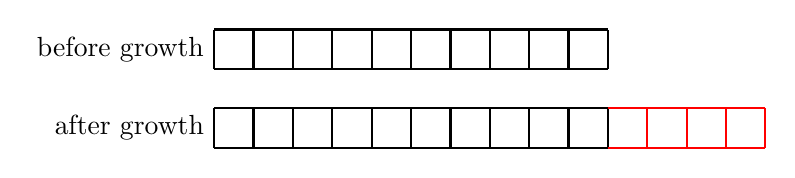
\begin{tikzpicture} [field/.style = {thick,step=5mm} ]
    \draw[field] (0mm,0mm) node[anchor = east,yshift=+2.5mm] {before growth} grid (50mm,5mm); 
    \draw[field] (0mm,-10mm) node[anchor=east,yshift=+2.5mm] {after growth} grid +(50mm,5mm);
    \draw[field,color=red] (50mm,-10mm)  grid +(20mm,5mm);
    \end{tikzpicture}
\end{minipage}
\caption{{\small\label{fig:field:growth1d} Growing a one dimensional field 
by $4$ elements.}}
\end{figure}
%%%---------------------------------------------------------------------------

%%%---------------------------------------------------------------------------
\begin{figure}[tb]
    \begin{minipage}[c]{0.3\linewidth}
        \begin{cppcode}
h5::nxfield f = ...;
//..... code omitted .....
f.grow(1,4);
        \end{cppcode}
    \end{minipage}
    \hfill
    \begin{minipage}[c]{0.65\linewidth}
        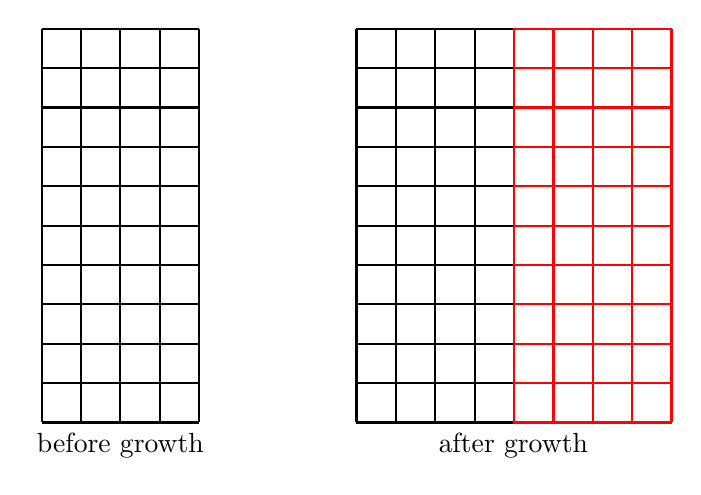
\begin{tikzpicture} [field/.style = {thick,step=5mm} ]
        \draw[field] (0mm,0mm) node[anchor = north,xshift=10mm] {before growth} grid (20mm,50mm); 
        \draw[field] (39.9mm,0mm) node[anchor=north,xshift=20mm] {after growth} grid +(20mm,50mm);
        \draw[field,color=red] (59.9mm,0mm)  grid +(20.1mm,50mm);
        \end{tikzpicture}
    \end{minipage}
    \caption{{\small\label{fig:field:growth2d} Growing a two dimensional field
    by $4$ elements along its second dimension.}}
\end{figure}
%%%---------------------------------------------------------------------------
The reason why there are no purely scalar fields is that during an experiment 
one would append data to a field as the measurement progresses. 
For this purpose \nxfield\ provides a \cpp{grow()} method which allows to 
extend the field along a particular dimension. The member function has the 
signature
\begin{cppcode}
void grow(size_t e,size_t n=1)
\end{cppcode}
where the first (mandatory) argument is the index of the dimension along which
the field should grow and the second (optional) argument contains the number of 
elements by which to grow. Figures~\ref{fig:field:growth1d} and
\ref{fig:field:growth2d} show examples of growing a one and a two dimensional
field respectively.

The canonical application for this feature would be to add content to a field 
as an experiment progresses. Using such a pattern we can start with a field 
of $0$ size and then add points if required. The principal code would look like
this
\begin{cppcode}
h5::nxfile f = ...;
h5::nxfield data = detector_group.create_field<uint16>("spectra",
                                                       shape_t{0,1024});
size_t index = 0;
while(true)
{
    data.grow(0,1); //grow by one element along first dimension
    //...... code omitted ....
}
\end{cppcode}
Note here that the initial shape of the field is $(0,1024)$. Such a pattern 
removes the burden of determining the number of points, recorded during 
an experiment, before the experiment starts. If the measurement is stopped 
somewhere in between the number of points written to the file matches exactly
the number of points recorded.  
It is important to note that one cannot extend the size of a field only along
\emph{existing} dimensions. It is not possible to change the rank of a field via
the growth method. Every attempt to do so will raise an \cpp{index\_error}
exception.
How to write the data will be explained in the next section.

%%%===========================================================================
\subsection{Partial reading and writing}

The previous section explained how to adjust the size of fields dynamically. 
What is still missing is how to write data to such a growing field. The 
\cpp{read()} and \cpp{write()} member functions used so far are always writing
the entire content of the field. This is not really what we want. 
Thus, \libpniio s \nxfield\ type provides partial IO quite similar to the 
\cpp{mdarray} template of \libpnicore. 

The best way to understand partial IO is to have a look on an example. We thus
will complete the previous one 

\begin{cppcode}
h5::nxfile f = ...;
h5::nxfield data = detector_group.create_field<uint16>("spectra",
                                                       shape_t{0,1024});
auto buffer = dynamic_array<uint16>::create_array(shape_t{1024});

size_t index = 0;
while(true)
{
    data.grow(0,1); //grow by one element along first dimension
    //...... code omitted ....

    //write data
    data(index++,slice(0,1024)).write(buffer);
}
\end{cppcode}
The important line of code here is the last one in the \cpp{for}-loop. To obtain
a selection of a field we can use the \cpp{()} operator of \nxfield. 
The selection works the same as for \cpp{mdarray}. However, the return value is 
a new field instance with the selection set. One currently cannot apply more
selections successively. 


%%%===========================================================================
\subsection{Field inquiry}\label{section:field:inquiry}

Fields share a set of inquiry functions with groups. These are \cpp{name()}, 
\cpp{filename()}, and \cpp{is\_valid()}. In addition to these functions
there are also some member functions which are special for fields. 
The \cpp{size()} member function returns the total number of elements 
stored in a field. If a selection has been applied to the field \cpp{size()}
returns the total number of elements selected. 
\cpp{type\_id()} returns the Id of the field elements data type. 
The \cpp{shape()} template function returns a container, which can be passed as
a template parameter, with the number of elements along each dimension. 
\begin{cppcode}
h5::nxfield field = ...;
auto s = field.shape<shape_t>();
\end{cppcode}



%%%===========================================================================
\section{Working with attributes}

Attributes are quite similar to fields. They can be attached to either a group
or a field to provide additional information (metadata) for a particular field
or group. Unlike fields attributes cannot 
\begin{itemize}
\item use compression
\item grow.
\end{itemize}
HDF5 attributes also do not support partial IO. However, \libpniio\ provides
partial IO for attributes in its implementation.
Attributes can be accessed from their parent object (field or group instance)
via the public attribute \cpp{attributes}. \cpp{attributes} is an instance of 
the \cpp{nxattribute\_manager} template class. The details about
\cpp{nxattribute\_manager} is only of interest for developers working on
\libpniio\ and hence will not be discussed here. Only the interface
\cpp{nxattribute\_manager} exposes is of interest and will be discussed in this
section. 

%%%===========================================================================
\subsection{Creating attributes}

Attributes are created via the \cpp{create()} template member functions 
provided by \cpp{nxattribute\_manager}. These functions are quite similar to
those used to create fields below groups. 
\begin{cppcode}
h5::nxfield f = ....;
auto units = f.attributes.create<string>("units");
\end{cppcode}
This short snippet creates an instance of \cpp{nxattribute} the template 
type used to represent attributes in memory. The newly created attribute 
is scalar and can store a single string. 
Multidimensional attributes can be constructed by adding a container with 
shape information to the argument list of the \cpp{create} template.
\begin{cppcode}
h5::nxfield f = ...;
auto matrix = f.attributes.create<float32>("transformation",shape_t{3,3});

std::cout<<matrix.rank()<<std::endl; //output is 2
\end{cppcode}
It is important here to note that even a scalar attribute has a rank of $1$. 
This might not be the obvious choice but makes fields and attributes more 
consistent. To check if an attribute is a scalar one could use the \cpp{size()}
member function of an attribute. If the \cpp{size()} returns $1$ the attribute
can be considered as scalar.

When one tries to create an attribute on an object which already has an
attribute of the same name an \cpp{object\_error} exception will be thrown. 
\begin{cppcode}
h5::nxfield f = ....;
f.attributes.create<string>("units"); //create the original attribute
f.attributes.create<float32>("units"); //would throw object_error
\end{cppcode}
However, an attribute can be overwritten with 
\begin{cppcode}
h5::nxfield f = ....;

//create the original attribute
f.attributes.create<string>("units"); 

//overwrite original attribute
f.attributes.create<float32>("units",true); 
\end{cppcode}
where the last argument of the second call to \cpp{create()} allows to 
overwrite an existing attribute. A similar call exists for multidimensional 
attributes
\begin{cppcode}
h5::nxfield f = ....;

//create the original attribute
f.attributes.create<string>("units",shape_t{3});       

//replace the original "units" attribute
f.attributes.create<float32>("units",shape_t{3,4},true); 
\end{cppcode}

%%%===========================================================================
\subsection{Attribute inquiry}

Attributes and fields share the same set of inquiry methods. Thus, see 
Section~\ref{section:field:inquiry} for details.

%%%===========================================================================
\subsection{Accessing an objects attributes}

The attribute manager instance associated with each field or group exposes a
very minimalistic but STL compliant container interface. 
Its \cpp{size()} returns the number of attributes attached to an object. 
One can access each attribute either by its index
\begin{cppcode}
h5::nxgroup g = ....;

for(size_t i=0;i<g.attributes.size();++i) 
    std::cout<<g.attributes[i].name()<<std::endl;
\end{cppcode}
or by its name
\begin{cppcode}
h5::nxgroup g = ....;
auto attr = g.attributes["NX_class"];
\end{cppcode}
When using the \cpp{[]} operator with a numeric index an \cpp{index\_error}
exception will be thrown if the index exceeds the total number of attributes. 
Similarly, \cpp{[]}, when used with an attributes name, will throw a
\cpp{key\_error} exception.
One can also iterate over all attributes, either by using the standard 
\cpp{begin()} and \cpp{end()} functions to retrieve iterators, or by using the
more modern for-each construction
\begin{cppcode}
h5::nxfield f = ....;
for(auto attr: f.attributes)
    std::cout<<attr.name()<<std::endl;
\end{cppcode}


%%%===========================================================================
\subsection{Reading and writing data from and to attributes}

Data IO for attributes works exactly the same as for fields with the exception
that attributes cannot be changed in size. 
A simple example for writing and reading a string attribute would look like this
\begin{cppcode}
string unit = "nm";
h5::nxfield f = ....;
auto attr = f.attributes.create<string>("units");
attr.write(unit);
//...... code omitted ......
attr.read(unit);
\end{cppcode}
The read/write member functions also accept instances of the \cpp{mdarray}
template as well as of \cpp{array}. Like for fields a pointer version exists 
to interact safely with legacy C libraries
\begin{cppcode}
size_t size = 9;
double *matrix = get_matrix_from_c_code();

h5::nxfield f = ....;
auto attr = f.attributes.create<float64>("matrix",shape_t{3,3});
attr.write(n,matrix);
\end{cppcode}
Reading works pretty much the same, however, you have to allocate memory before
reading the data from the attribute
\begin{cppcode}
h5::nxfield f = ....;
auto attr = f.attributes["matrix"]; //obtain the attribute from the field
float64 *matrix = allocate_memory(attr.size());

attr.write(attr.size(),matrix);
\end{cppcode}
Unlike standard HDF5 attributes support \libpniio's \nexus-attributes partial
IO. Partial IO with attributes works exactly the same way as with field
\begin{cppcode}
h5::nxfield f = ...;
auto attr = f.attributes.create<float64>("matrix",shape_t{3,3});
auto row  = dynamic_array<T>::create(shape_t{3});
//........... code omitted .......
for(size_t i=0;i<3;++i)
{
    row = .....; //fill row buffer with data
    attr(i,slice(0,3)).write(row);
}
\end{cppcode}
For reading data just replace the \cpp{write} with \cpp{read}. It should be
mentioned that using partial IO on attributes, though it works, can be
significantly slower than writing the entire attribute in a single step. 

%%%===========================================================================

\subsection{Attribute management}

There are two functions left of the \cpp{nxattribute\_manager} interface. 
One is the \cpp{exists()} member function which can be used to check for the
existence of a particular attribute. 
\begin{cppcode}
if(!field.attributes.exists("units"))
    std::cerr<<"Field does not have a units attribute!"<<std::endl;
\end{cppcode}
An attribute can be removed from an object using the \cpp{remove()} method. 
\begin{cppcode}
if(field.attributes.exists("units"))
    field.attributes.remove("units");
\end{cppcode}
The \cpp{remove} method throws \cpp{key\_error} if the attribute to delete does
not exists.


%%%===========================================================================
\section{Working with links}

%%%---------------------------------------------------------------------------
\begin{figure}
\centering
\begin{tikzpicture}
    \node[nxgroup] (entry) {\nodepart{one} entry \nodepart{two} \nxentry};
    \node[nxgroup,right = of entry] (instrument) {\nodepart{one} instrument 
                               \nodepart{two} \nxinstrument};
    \node[nxgroup, right = of instrument] (detector) {\nodepart{one} detector
                             \nodepart{two} \nxdetector};
    \node[nxfieldh=5, right = of detector] (detectordata) 
                                        {\nodepart{one} data
                                         \nodepart{two} $1.2$ 
                                         \nodepart{three} $4.3$ 
                                         \nodepart{four} $7.89$ 
                                         \nodepart{five} \dots
                                         };
    \node[nxgroup, below = of instrument] (data) {\nodepart{one} data
                         \nodepart{two} \nxdata};
    \node[nxfieldh=2,right = of data] (datalink)
                                   {\nodepart{one} data
                                    \nodepart{two}
                                    \texttt{../instrument/detector/data}
                                   };

    \draw[thick,->] (entry.east) -- (instrument.west);
    \draw[thick,->] (instrument.east) -- (detector.west);
    \draw[thick,->] (detector.east) -- (detectordata.west);
    \draw[thick,->] ($(entry.east)!0.5!(instrument.west)$) |- (data.west);
    \draw[thick,->] (data.east)--(datalink.west);
    \draw[thick,dashed,->] (datalink.north) --
                           node[midway,right] {link}
                           (detectordata.south west);
\end{tikzpicture}
\caption{{\small\label{fig:link:internal_link}
Links can be used to make data available in two different group without
duplicating the data. Here the data stored in the detector is also available
below the data group in the entry group of the tree. 
}}
\end{figure}
%%%---------------------------------------------------------------------------

%%%---------------------------------------------------------------------------
\begin{figure}
    \centering
    \begin{tikzpicture}[level distance = 2cm]
        \node[nxgroup] (master entry) { entry \nodepart{two} \nxentry}
          [growth parent anchor = north east] 
          child { 
                  node[nxgroup] (master instrument) {instrument 
                                               \nodepart{two} \nxinstrument}
                  child {
                    node[nxgroup] (master detector) { detector
                                               \nodepart{two} \nxdetector}
                      child{
                        node[nxfieldv=2] (master link) { data \nodepart{two} 
                        \texttt{\tiny
                        detector.nxs://entry/instrument/detector/data} 
                        }
                      }
                  }
                };

         \node[nxgroup,right = 7cm of master entry] (detector entry) 
                 { entry \nodepart{two} \nxentry}
          [growth parent anchor = north east] 
          child { 
                  node[nxgroup] (detector instrument) {instrument 
                                               \nodepart{two} \nxinstrument}
                  child {
                    node[nxgroup] (detector detector) { detector
                                               \nodepart{two} \nxdetector}
                      child{
                        node[nxfieldv=2] (detector data) 
                        { data \nodepart{two} 
                          \begin{tikzpicture}
                          \draw[step=1mm] (0,0) grid (20mm,5mm); 
                          \end{tikzpicture}
                        }
                      }
                  }
                };
        
            \draw[thick,dashed,->] (master link.south) .. 
                                   controls ($(master link.south)!0.1!(detector
                                   data.south)+(0cm,-1.5cm)$) and 
                                   ($(master link.south)!0.9!(detector
                                   data.south)+(0cm,-1.5cm)$)
                                   .. node[midway,below]{external link}(detector data.south);

            \begin{scope}[on background layer]
                \node[rectangle, draw,rounded corners,fit=(master entry)(master
                link)] (master file){};
                \node[above = 0.25cm of master file,align=center] {\nexus\
                master file\\ \texttt{master.nxs}};
                \node[rectangle, draw,rounded corners,fit=(detector entry)
                (detector data)] (detector file) {};
                \node[above = 0.25cm of detector file,align=center] 
                {\nexus\ detector file\\ \texttt{detector.nxs}};
            \end{scope}
    \end{tikzpicture}
    \caption{{\small\label{fig:link:external_link}
    An external link used to reference the data stored in a separate detector
    file via the data field in the master file. The master file is what the user
    typically uses to access the data. 
    }}
\end{figure}
%%%---------------------------------------------------------------------------

One of the key features of \nexus\ is its support for links. Like on a file
system linking allows for making data available at different positions in the
\nexus\ group hierarchy without data duplication. 
A typical application for a link would be the data stored in \nxdata\ instance
of a \nexus-file. \nexus\ distinguishes two kinds of links
\begin{itemize}
\item internal links - where the link and its target are located in the same
file
\item and external links - where the target resides in a different file than the 
link.
\end{itemize}
For both kinds of links there are canonical use cases. 
The standard use case for internal links is depicted in
Fig.~\ref{fig:link:internal_link}. Here the link is used to reference the data
stored in the detector group of the file in its data group\footnote{This group
is used for programms to quickly find plottable data.}.
By using links we only have to store the data once (in the detector group) and
can make it available at any other position in the file.

The default use case for external links is shown in
Fig.~\ref{fig:link:external_link}. In many cases detector write to a network
storage while entirely bypassing the control system of the experiment. This is
typically done when the detector has to record images hat a very hight rate
which could not have been achieved if all the data has to be pumped through the
control systems software stack. 
In the best case, as shown in Fig.~\ref{fig:link:external_link}, the detector
already writes its data in a \nexus\ file which contains nothing else than the
detector images. While the detector is recording images the control system
writes all the metadata and other relevant data to a master file (this data is
usually rather small and not recorded at low frequency). As a result we end up
with two files and the user would have to access metadata through the master
file and the detector images via the detector file. By using external links 
it is possible to make data within a \nexus-file availabe that is originally
stored in a different \nexus-file. Now the user can access the detector data via
the master file as it would be stored directly within this file.
The only thing the user has to remember is that he or she needs to copy two
files when movin the data to a different storage.

%%%===========================================================================
\subsection{Create internal links}

To create an internal link the \cpp{pni::io::nx} namespace provides the
\cpp{link()} function template which exists in several overloaded versions.
All of them differ virtually only in the way how the link target is referenced
which is the first argument of \cpp{link()}. The second and third argument are
the parent group for the new link and its name.

The most intuitive version of the \cpp{link()} function template references the
target object directly via their group or field instance. The next example shows
the canonical case where a new link to the detector data is generated below the
data group. 
\begin{cppcode}
h5::nxfile  f          = h5::nxfile::open_file(data,true);
h5::nxgroup entry      = f.root()["entry"];
h5::nxgroup instrument = entry["instrument"];
h5::nxgroup detector   = instrument["detector"];
h5::nxgroup datagroup  = entry["data"];
h5::nxfield det_data   = detector["data"];

link(det_data,data_group,"data");
\end{cppcode}
With this approach only internal links can be created as the target and the
parent object for the new link must be located in the same file. 
This approach is rather tedious as we have to open all the groups (for now we
have no better way - see the advanced section). However, one can exploit a
feature that \nexus-links have in common with file system links: the target
object must be available when the link is created. Consequently we can describe
the target also merely by its path
\begin{cppcode}
h5::nxgroup data_group = ...;

link("../instrument/detector/data",data_group,"data");
\end{cppcode}
Here the first argument (the target) is described by a string with the path to
the target. In this case the path is relative to the parent group of the link. 
Alternatively one can also use an instance of \cpp{nxpath} to reference the 
target object
\begin{cppcode}
h5::nxgroup data_group = ....;
nxpath target_path = nxpath::from_string("../instrument/detector/data");

link(target_path,data_group,"name");
\end{cppcode}
There is one important restriction a path has to obey when it should be used as
a reference to a link target: the path must not contain type only elements. 
For instance the path \cpp{"../:NXinstrument/:NXdetector/data"} would be a
perfect valid \nexus-path. However, when using such a path \cpp{link} will throw
a \cpp{value\_error} exception. The reason for this is simple: \libpniio\
currently uses the HDF5 linking mechanism which has no idea about \nexus-group
types!
Thus, as a rule of thumb, use only names within the path used to reference a
link target.

There is some other subtle issue with paths to link targets. They must not
comprise intermediate parent directory references (\cpp{..}). 
This cannot be handled by HDF5 correctly. \cpp{..} is only allowed at the 
beginning of a relative path. Absolute paths must not contain any \cpp{..} 
elements. 
Thus \cpp{../../entry/instrument} would be a valid target path for a link, 
but \cpp{/../entry/../entry} would not. 

%%%===========================================================================
\subsection{Create external links}

To create external links within a \nexus-file use the \cpp{link} function as for
internal links. However, only the string and path version of \cpp{link} can be
used to create external links. 
The only thing one has to do in order to obtain a link add the filename to the
path. Lets start again with the canonic example, the external detector file
\begin{cppcode}
h5::nxgroup detector_group = ....; //open the detector group in the master file

link("detector.nxs://entry/instrument/detector/data",detector_group,"data");
\end{cppcode}

%%%===========================================================================
\subsection{Link inquiry}

\libpniio\ (or better HDF5) distinguishes three kinds of links
\begin{inlinetab}{m{0.3\linewidth}m{0.5\linewidth}}
hard links & these are links to an object which are typically created 
             from the parent object to a newly created field or group \\
soft links & this is what one typically creates with the \cpp{link} function
template \\
external links &  are links that reference an object in a different file.
\end{inlinetab}
The major difference between hard- and soft-links is the fact that the latter
ones can dangle (the object they point to must not exist). 
\libpniio\ provides utility functions to check what kind of link one deals with. 
\begin{cppcode}
h5::nxgroup parent = ...;
string name = "data";

if(is_hard_link(parent,name))
    std::cout<<"hard link";
else if(is_soft_link(parent,name))
    std::cout<<"soft link";
else if(is_external_link(parent,name))
    std::cout<<"external link";
else
    std::cout<<"unkown link type";
\end{cppcode}
Each of the function takes the parent object of the link as its first and the
name of the link as its second argument. 





